\chapter{A long, long way}
\newpage
\section{A long long way}
Consider an adjective like \data{long}. Simply by repeating it, we manage to amplify its meaning, essentially doubling down on it. This is effect when The Hollies sing:

\begin{quote}
\data{It's a long, long road}\\
\data{From which there is no return}
\end{quote}

\noindent The reduplicative use of \data{long} emphasizes the sheer immensity of the journey in a way that would not come across at all if the lyric were the more prosaic \textit{it's a long road}.

Another verse, though, goes like this:

\begin{quote}
\data{The road is long}\\
\data{With many a winding turn}
\end{quote}

Now imagine reduplicating \data{long} here. Far from adding emotional depth, it would just be ridiculous. Nobody says *\data{the road is long long}. And what's fascinating is that we all intuitively grasp the difference between these two superficially similar uses of repetition. Why would that be? Is there a universal rule at play, or is it something peculiar about the structure of English?

When I say we all grasp the difference, I'm including people who have only the most limited grasp of English. Geoff \citet{pullum2006} mentioned the case of a Turkish woman saying of the pope in 2006, *\data{John Paul very very good}. Here's a woman whose grasp of English is so limited (though far better than my grasp of Turkish) that she omits \data{is}, and yet she nevertheless seems to know that you can convey the depth of the pope's goodness by reduplicating \data{very}. Pullum thinks this suggests the woman might be simply repeating something she's heard before, either in English or Turkish. 

It seems unlikely that she's heard it in English, though. The string \textit{very very} appears only about two and a half times per million words, about half as often as a word like \textit{levy} or \textit{whereby}. It's almost certain that she's directly imported the structure from Turkish, a process called \textsc{calquing}. \textit{That's \uline{very very} good} is \textit{Bu \uline{çok çok} iyi} in Turkish.

But I wonder if something more is going on here. I teach English to international students studying in Canada, some of them beginners, and I've given them examples like \data{a long long road} and \data{the road is long long}. There's never any reaction after the first, but laughter inevitably follows the second in a way it never does with other grammatical infelicities. These students just know that it's wrong.

\begin{tcolorbox}[title=Breaking it down, colback=white, parbox] \label{sec:long-long}
\setlength{\parindent}{1.5em}

Let's take a moment to dissect this construction. The phrase \data{a long road} is a noun phrase, where \data{road} is the head noun and \data{long} is an adjective functioning as a modifier. More specifically, \data{long} is an attributive modifier, a modifier that precedes the head noun, assigning it a particular property, in this case, the attribute of length.

In contrast, \data{the road is long} is a clause. While \data{long} remains an adjective, its function has changed. It's not complement in the clause, not a modifier. To be specific, it's a predicative complement, one appearing after a verb and conveying what is said of, or ``predicated'' of, the subject (\data{the road}). Other predicative complements are \textit{you're \uline{beautiful}}, \textit{they all seem \uline{so happy}}, or \textit{I feel \uline{good}}.

Finally, the doublet \textit{long long} exemplifies a construction called \textsc{reduplicative intensification}, ``reduplicative'' because it is doubled, and ``intensification'' because it strengthens the meaning of the original adjective.

\end{tcolorbox}

With this analysis under our belts, we can attempt a general statement about reduplicative intensification in English.%, though we will want to revise this later:

\ea[]{An adjective in attributive modifier function in a noun phrase may be repeated with the effect of intensifying its meaning. This is not possible in other functions, such as predicative complement.}\label{def:reduplication-rule}
\z

We've seen that something like (\ref{def:reduplication-rule}) is true in English, but what about other languages. Intriguingly, the same statement often seems to hold. For example, Japanese has

\ea
   \ea[]{
        \gll 長い  長い  道\\
        nagai nagai michi\\
        \glt ‘a long long road’}
   \ex[*]{
        \gll 道     が 長い 長い\\
        michi ga nagai nagai\\
        \glt ‘the road is long long’}
   \z
\z


And in Russian we find
\ea
    \ea [ ] {
        \gll красивые, красивые глаза\\
        krasivye, krasivye glaza\\
        \glt `beautiful, beautiful eyes'}
    \ex [*] {
        \gll Её глаза красивые, красивые\\
        Yeyo glaza krasivye, krasivye\\
        \glt `her eyes are beautiful beautiful'}
    \z
\z


%\ea [] 
%    \ea
%        {\gll  \\
%        nagai nagai michi \\
%        \trans `a long long road'
%        }
%    \ex [*]
%        {\gll  \\
%        michi \textsc{Subj} nagai nagai \\
%        trans `the road is long long' \\
%        }
%    \label{ex:長い長い}
%\z\z

%\a
%\gll 長い 長い 道 \\
%nagai nagai michi \\
%\trans `a long long road'
%\b
%\gll 道 が 長い 長い \\
%michi \textsc{Subj} nagai nagai  \\
%\trans `the road is long long'
%\z\z

%One modification we might want to make to (\ref{def:reduplication-rule}) is to constrain the set of adjectives to which it applies. Adjectives like \data{long} and \data{old} pick out the scalar properties of length and age. We can put them on a scale and measure or at least rank them. But not all adjectives lend themselves to such ranking. A fossil from the Cambrian period is a Cambrian fossil and other fossils are just not. There is no scale of Cambrianicity on which we can place them. As a result, *\data{a~Cambrian~Cambrian~fossil} is ruled out.

Why should (\ref{def:reduplication-rule}) hold? Why is intensificatory reduplication possible for adjectives functioning as attributive modifiers, but not in other functions. We might speculate that there is some property of the human mind makes this construction impossible in predicative functions. This would explain the pattern we see across languages but would be ruled out by finding a language that allowed the construction in predicative complements. Or it might be that there is something about the meaning of \textit{long long} that changes when it's in the predicate, a difference that does not apply to other ways of boosting the adjective's meaning such as \textit{it's a very long road} or \textit{the road is very long}. On the other hand, it might just be a historical accident.


\subsection{Old English}

Intensificatory reduplication didn't exist in Old English. In fact, an Old-English speaker couldn't even put two adjectives back to back for the most part. *\textit{Micel blæc fugol} `big black bird' would have been ungrammatical because the adjectives \textit{micel} and \textit{blæc} couldn't appear together like that. Instead, it might have been rephrased as \textit{micel fugol \& blæc} `big bird and black'. But just because you couldn't string two adjectives together doesn't mean you couldn't have two modifiers side by side. You just had to sneak one inside the noun.

\textit{Blackbird} is a Modern-English compound, a noun made up of two words: the modifier \textit{black} and the head noun \textit{bird}. We think of compounds like \textit{blackbird} as single words because their meaning changes if you take them apart. A black bird is a bird that is black, but female blackbirds are often brown. A raven is a black bird, but it is most certainly not a blackbird. So, although the adjective \textit{black} is a modifier in the compound, it's is invisible to the surrounding grammar. To illustrate, we can say \textit{a \ob really black\cb~bird} but not *\textit{a really blackbird} because \textit{really} can't ``see'' \textit{black}.

\begin{figure}
    \centering
    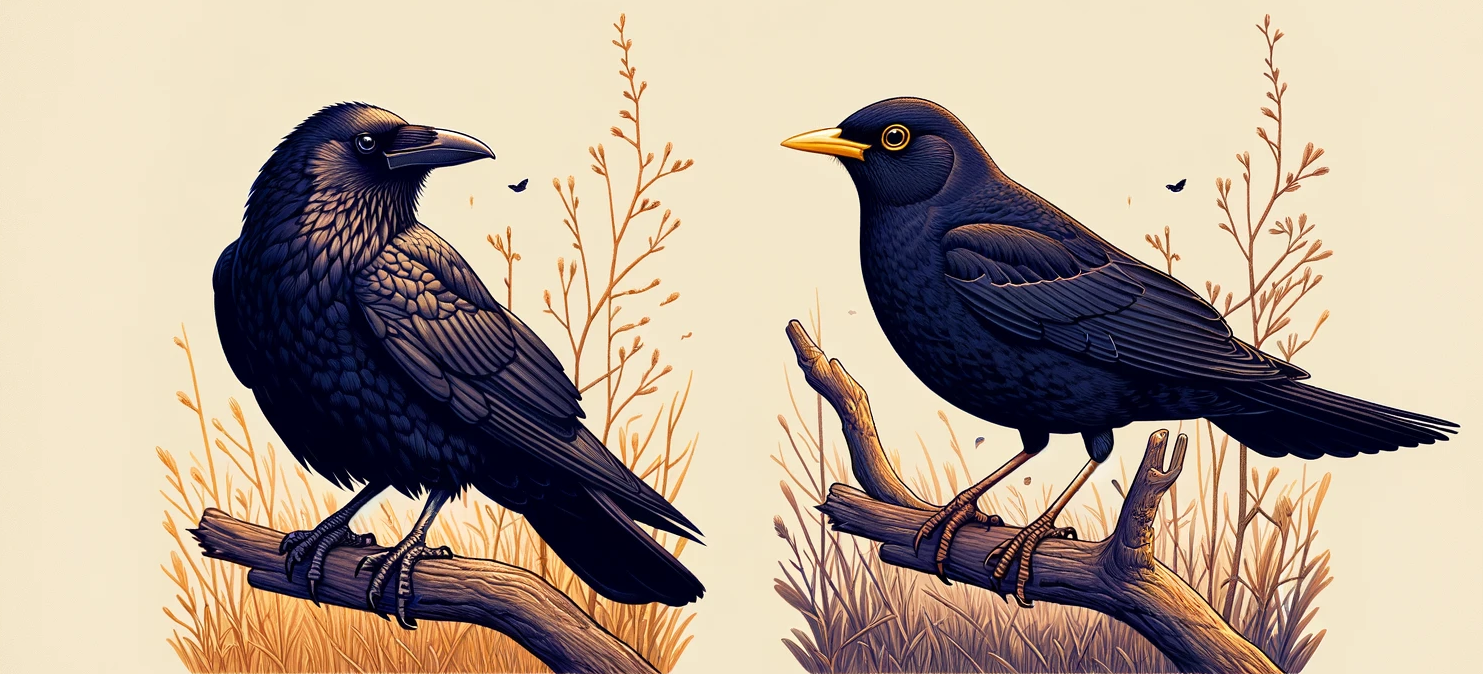
\includegraphics[width=\textwidth]{figures/black-birds.png}
    \caption{A black bird and a blackbird. Image by DALL$\cdot$E.}
    \label{fig:black-birds}
\end{figure}

Although we don't find *\textit{citygate} today, \textit{burggeat} was a compound noun in Old English, made up of the modifier \textit{burg} `town/city' and the head noun \textit{geat} `gate'.  And just as \textit{really} can't ``see'' \textit{black} in \textit{blackbird}, an attributive modifier like \textit{micel} `great' would have been insensitive to \textit{burg} in \textit{burggeat}. With \textit{burg} tucked safely inside the compound noun, \textit{\uline{micel} \uline{burg}geat} wouldn't have felt like two modifiers in a row.

\begin{figure}
    \centering
    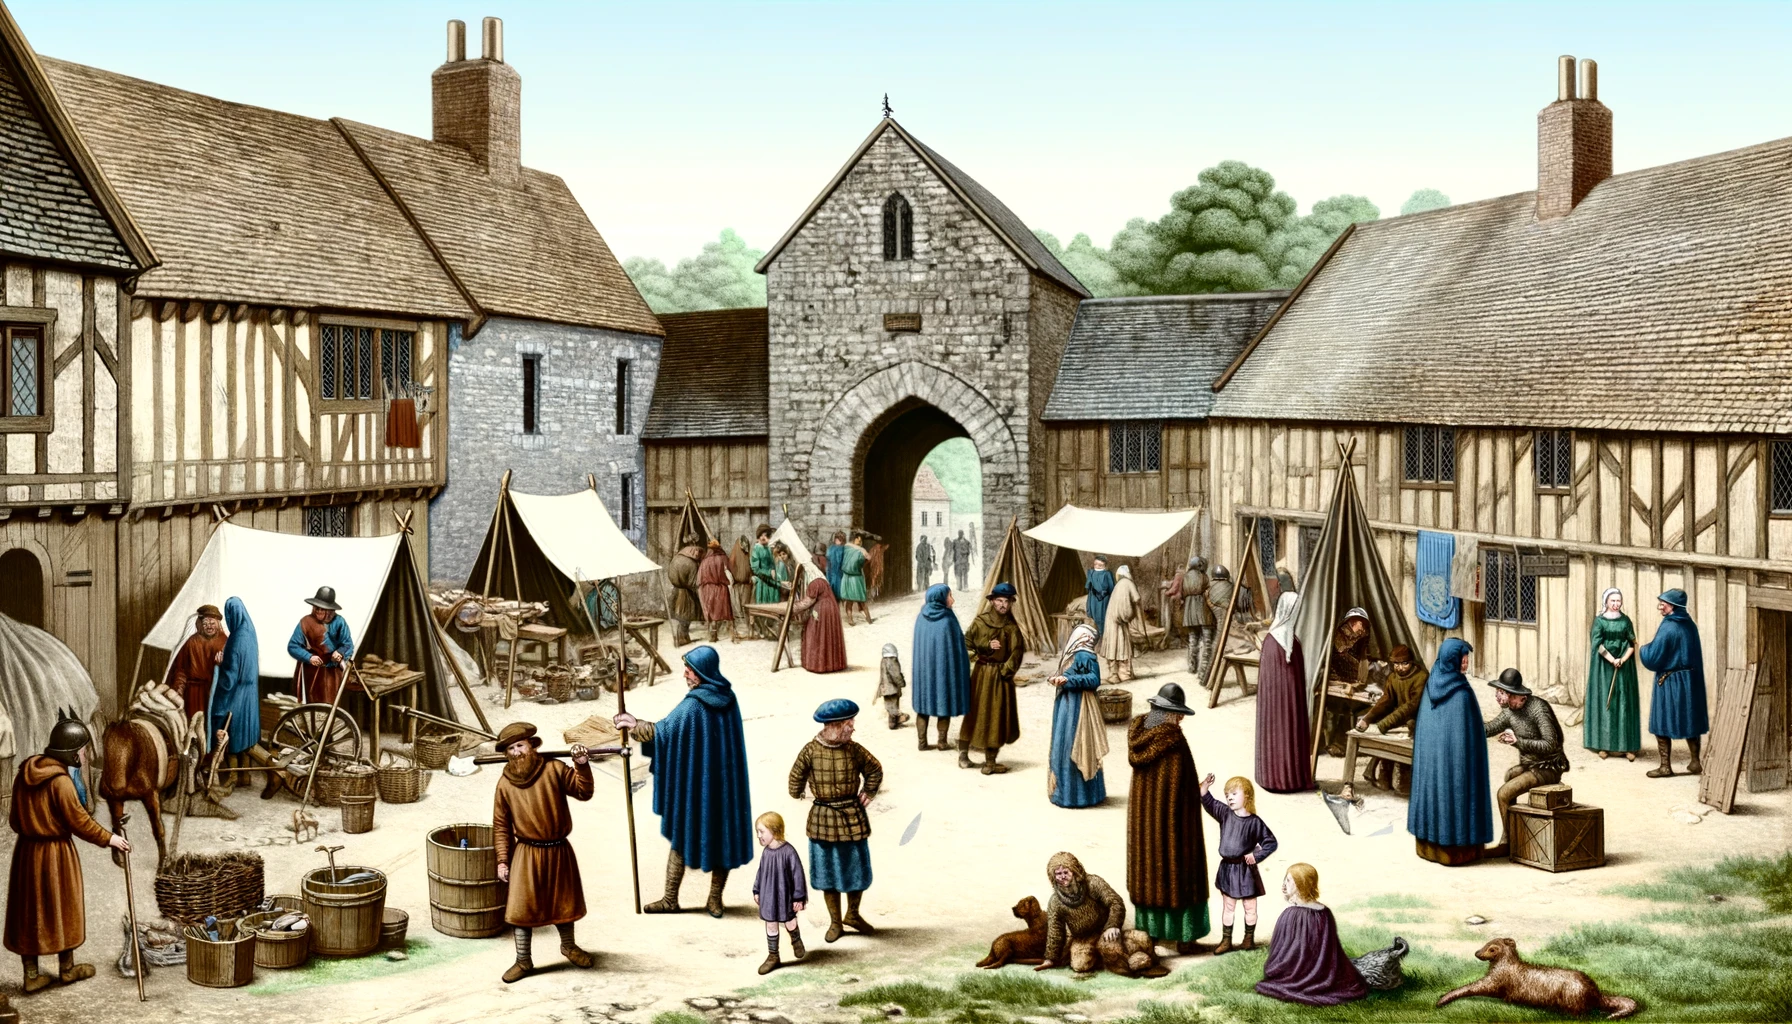
\includegraphics[width=\textwidth]{figures/DALL·E-burggeat.png}
    \caption{Folks near a burggeat. Image by DALL$\cdot$E.}
    \label{fig:burggeat}
\end{figure}

%Once a compound noun like this was available, the process could be repeated: \textit{setl} is a seat or throne, and so a \textit{burggeatsetl} is a `city-gate-seat', a place where, for instance, trials could be held. At first blush, this looks like multiple adjectives -- after all, there's the head noun \textit{setl} on the right, and there are two modifiers before it -- but this is a red herring in two ways. The first, I hope, is clear. Despite being modifiers \textit{burg} and \textit{geat} are not adjectives. The second is that \textit{setl} has one modifier, not two. \textit{Burg} modifies \textit{geat}, not \textit{setl}, and only then does \textit{burggeat} modify the head noun, like this: [\textit{\ob\ob burg\cb geat\cb setl}].

Nevertheless, the odd burgher may have interpreted \textit{burggeat} as two words instead of one, and so for them \textit{micel burg geat} would have had two contiguous modifiers. It's only a short step from \textit{micel burg geat} `great city gate' to something like \textit{micel blæc geat} `great black gate' or \textit{fæst eald geat} `strong old gate'. Not only would that have put two modifiers in a row, but both of the modifiers would have been adjectives.

%In Old English, adjectives as modifiers could appear before the noun or after (e.g., \textit{englum halgum} `with holy angels'), but when it came to noun compounding, the modifier-first was the rule. A city gate could only be \textit{burggate} not *\textit{gateburg}.

%The compound noun (modifier + head) itself could be modified by an adjective. \textit{micel burggeat} meant `(the) great city gate'. While these aren't back-to-back adjectives, they are back-to-back modifiers. And they're only possible to the left of the noun because the modifier within the compound comes before the head.

In our story so far, Old-English grammar was quite restrictive compared to Modern English. Two adjectives couldn't be strung together to modify a noun directly. However, compound nouns may have provided a workaround. Since elements within a compound noun are treated as a single unit, they allowed for a modifier to be placed in front of this unit (like \textit{great} in \textit{great city gate}). This structure may have gradually eroded the restriction on multiple adjectivie modifiers, eventually making it possible to have noun phrases such as \textit{\uline{micel blæc} geat} `great black gate'. It did nothing, though, to change the limit on multiple adjectives in other contexts like *\textit{the gate was \uline{great black}}.

%\begin{center}
%    -- --
%\end{center}

%Next, adjectives and nouns could share a shape. A modern example is \textit{deep}, which is usually an adjective but is a noun in \textit{the deep of space}. An example from Old English is \textit{īsern} `iron'. As a noun, it could appear in compounds, such as \textit{īsernbȳrne} `iron breastplate or corselet', and as an adjective, it could be a pre-head modifier, as in \textit{īserna helm} `iron helmet'. That final -\textit{a} marks this clearly as an adjective, but the adjective didn't always have this -\textit{a}. In other cases, it shared the form \textit{īsern} with the noun. This sets up the possibility for people to see \textit{godra īsernbȳrne} `(a) good iron breastplate' as having multiple adjectives both ultimately modifying the head \textit{bȳrne}.

%Another construction that motivates the possibility of multiple pre-head adjectives is modification for number or possession. In Old English, there wasn't a proper determiner function in the way there is in Modern English -- a noun phrase like \textit{īserna helm} `iron helm' didn't need an article -- but there was a possibility to give a count as in \textit{six crata} `six chariots'. Importantly, this didn't ``use up'' the adjective's modifier spot; both could appear together, as in (\ref{ex:six-hundred}).

%\ea \label{ex:six-hundred}
%    \gll \textit{Farao} \textit{gegaderode} \uline{\textit{six} \textit{hundred} \textit{godra} \textit{crata}}\\
%        Pharaoh gathered {six hundred good chariots}\\
%    \glt `Pharaoh gathered six hundred good chariots.'
%\z

%Similarly, quantity words such as \textit{manig} `many', \textit{feawe} `few', \textit{eall} `all', and \textit{sum} `some' could precede an attributive adjective. Finally, possessives such as \textit{\uline{cyninges} īserna sweord} `(the) king's iron sword' were possible. Once again, these were only found to the left of the noun, never to the right. It shouldn't be surprising, then, if some speakers reinterpreted such cases as allowing not just multiple pre-head modifiers, but multiple pre-head adjectives. The predicative function had nothing like this.

\subsection{Middle English}

During the Middle English period, the language underwent dramatic changes. One involved the whole system of declension dropping away. This meant, for instance, that \textit{se hring} `the ring', which likely started Middle English like this

\begin{table}[h]
    \centering
    \begin{tabular}{|l|l|l|}
        \hline
        \textbf{Case} & \textbf{Singular}         & \textbf{Plural}          \\ \hline
        Nominative    & \textit{se hring}       & \textit{þā hringas}        \\ \hline
        Accusative    & \textit{þone hring}     & \textit{þā hringas}        \\ \hline
        Genitive      & \textit{þæs hringes}    & \textit{þāra hringa}      \\ \hline
        Dative        & \textit{þǣm hringe}     & \textit{þǣm hringum}      \\ \hline
    \end{tabular}
    \caption{Old English declension of \textit{se hring} `the ring'}
\end{table}

\noindent was flattened and simplified until it had been reduced to the four (arguably two) forms we know today:

\begin{table}[]
    \centering
        \begin{tabular}{lll}
        \hline
        \textbf{Case} & \textbf{Singular} & \textbf{Plural} \\
        \hline
        Plain & \textit{the ring} & \textit{the rings} \\
        Genitive   & \textit{the ring's} & \textit{the rings'} \\
        \hline
        \end{tabular}
    \caption{\textit{The ring} after the death of declensions.}
    \label{tab:gate-paradigm}
\end{table}

Those endings had signalled various noun functions. Without them, (\ref{ex:case-loss}) looks like the woman gave the queen a ring. With them, we can deduce that that the queen is the subject (nominative) and it was \textit{to} the woman (dative) that she gave the ring (accusative).

\ea \label{ex:case-loss}
    \gll \textit{Þām wife} \textit{sealde} \textit{sēo cwēn} \textit{hring}\\
        {the woman-DAT} gave {the queen-NOM} ring-ACC\\
    \glt `It was to the woman, that the queen give a ring.'
\z

As those endings eroded, speakers relied more on word order to tell the functions apart.  

At the same time, adjectives were becoming less distinct from other categories of words.

%In the more flexible order of Old English, it had been also possible for gentives like \textit{Joe's} to appear after the noun they modified, as in (\ref{ex:post-noun-genitive}).

%\ea \label{ex:post-noun-genitive}
%    \gll \textit{þa} \textit{digelnysse} \textit{þisre} \textit{rædinge}\\
%    the mystery this text-GEN\\
%    \glt `this text's mystery'
%\z

%. In the evolving situation of Middle English, the post-noun possessives fell out of favour, replaced by the \textit{of} structure we know today (e.g., \textit{the mystery \uline{of this test}}).  This shift could have reinforced the burgeoning idea that modifiers generally belong before the noun.

%The decline of the case system and the rise of a fixed word order in Middle English also coincided with a blurring of the lines between adjectives and other parts of speech. \citet[261]{Fischer2006a} notes that some of the earliest examples of two adjectives preceding a noun involve degree adjectives such as \textit{swiþe} `strong', \textit{ful} `full', \textit{riht} `proper, and \textit{verray} `true' (as in \textit{the very word of God}). For instance, \textit{the riht grete loue} means `the proper and great love'. But what if the listener interpreted \textit{riht} as an adjective, while the speaker intended it as an adverb, meaning `really great love' or `very great love'? This might encourage the hearer to update their credence in grammatical adjective--adjective pairs. In this case, though, it's less clear that any such reanalysis would favour the pre-head position.

All of this laid the groundwork for a new kind of intensification: redundant adjectives, as in (\ref{ex:gosefoote}; with minor spelling adjustments.)

\ea[]{\textit{gosefoote an evill herbe: it is called pes anserinus, leaved like night shade, but more jagged in the said leaves, bearing \ob \uline{small little} red flowers, with great plenty of seede, lyke unto arage\cb.}\\ \hfill (Bulleins bulwarke of defence against all sicknesse, 1579)}\label{ex:gosefoote}
\z

Not much later -- around the beginning of the 1600s -- examples of reduplicative intensification like \textit{a long long life} begin to show up reliably. \textit{Long} is one of the earliest words to participate in this construction, and it's still one of the most common.

At right around the same time, redoubled adverbs, such as \textit{very very good}, begin to appear. It may not be coincidental that \textit{long} is both an adjective and an adverb. Many of the early cases of \textit{long long} are adverbs such as \textit{long long sought-for love}.

In short, the ungrammaticality of *\textit{a tale which is old old} is more or less the historical default. It's what would have been the case if nothing had changed. On the other hand, it is only a long long chain of historical accidents on the left-hand side of the noun phrase that makes possible expressions like \textit{an old old tale}.

\subsection{In other languages}

Linguists often look for universals when observing cross-linguistic patterns like the one with reduplicative intensification. It turns out, though, that there is nothing inherently \textit{un}natural about post-head reduplicative intensificatory modification. We might not find it in English, Japanese, or Russian, but it's certainly out there. Geoff Pullum suggested I look at Jamaican Creole, and I found examples like (\ref{ex:blakblack}). 

\ea \label{ex:blakblack}
    \gll\textit{im} \textit{want} \textit{wan} \textit{we} \textit{blakblak}\\
    he wants one that black-black\\
    \glt `he wants one that is very black'\hfill\citep[129]{Gooden2003}.
\z

And when I looked further afield, I found others, such as (\ref{ex:qi-qilodo}) from North-East Ambae, an Oceanic language of Vanuatu.

\ea \label{ex:qi-qilodo}
    \gll \textit{Vai-gi} \textit{ngire} \textit{ra=u} \textit{qi-qilodo}\\
        do-become things those short-short \\
    \glt `Those things are very short.'\hfill\citep[278]{Hyslop2004}
\z

In other words, we're not programmed to prefer one kind of duplication over the other. We're socialized to do so.
     
\bigskip

What, then, could explain my English-language students producing examples like \textit{she good~good person} but laughing when I suggest ones like *\textit{she's good~good}?

Their production could very well be a generalization from their previous language experience, mirroring similar constructions in other languages, such as the Turkish example mentioned by Pullum.

As for their amusement at the predicative reduplication, my best guess is that they've extrapolated from the evidence they've seen in their time learning English that you simply don't find more than one adjective after \textit{is}. *\textit{She's nice good} would be as strange as *\textit{she's good good}. The problem is not specifically with reduplication.

\bigskip

In the 1970s, a new kind of adjective reduplication appeared, and this one can be prediative \citep{Gonzalez-Diaz2018}. It's a kind of compounding -- \textit{blackbird} vs \textit{black bird} -- and it's for clarification instead of intensification, for picking out the meaning that's not just right but that's \textit{right}-right. This could be the key that opens up other functions to multiple adjectives.

%As Middle English was giving way to Modern English in the 1600s, big complex noun phrases with multiple adjectives like \textit{\uline{big complex} noun phrases with multiple adjectives} or the one in (\ref{ex:gosefoote}) remained uncommon, but they did show up more and more, especially in certain genres, such as scientific and medical writing. ``In particular, it turns out that non-professional authors of medical texts were particularly prone to using excessive adjective sequences, often for the purpose of evoking strong responses in readers'' \citep[158--159]{Tyrkko2014a}.

%\ea[]{\textit{Blood, is \ob a \uline{hot, sweet, temperate, red} humour, prepared in the Miseriacke veins, and made of the most temperate parts of the Chilus in the liver\cb.} \phantom{............} \hfill(Burton, \textit{Anatomy of Melancholy}, 1621)}
%\z

%``By contrast,'' writes Tyrkkö, ``established medical authors writing for the professional community showed more restraint''. 

%Long strings of adjectives are uncommon, even today, but were even more rare at the time. In the corpus of medical texts, Tyrkkö finds only two strings of four adjectives as in 

%\ea[]{\textit{That which looketh of a \uline{pure transparent yellow amber} colour, like a pure sacke, is reputed the best. The best March beere, if well brewed, and no error committed, is often of this colour.} \hfill(Hart, Klinike, 1633)}
%\z

